\subsection{Расчет теплового режима РЭС в герметичном корпусе с внутренним перемешиванием}

В этом и последующих разделы формулы для расчетов идентичные таковым в
предыдущем разделе приведены не будут. Вместо этого записан результат
их вычисления с подстановкой свойственных конкретному расчету
значений.

\begin{enumerate}[label={\arabic*.}]
\item Рассчитывается поверхность корпуса блока~\cite{Rotkop1976}: % (4.46)
  $$S\mathrm{_{К}}=1,108\mathrm{м^2}$$
\item Рассчитывается условная поверхность нагретой зоны~\cite{Rotkop1976}: % (4.39)
  $$S\mathrm{_{з}} = 0,655\mathrm{м^2}$$ 
\item Находится удельная мощность корпуса блока ~\cite{Rotkop1976}:  % (4.45)
  $$q\mathrm{_к} = 13,53\mathrm{Вт/м^2}$$
\item Находится удельная мощность нагретой зоны ~\cite{Rotkop1976}: % (4.38)
  $$q\mathrm{_з} = 22,91 \mathrm{ Вт/м^2}$$

\item Определяется коэффициент $\vartheta_1$ в зависимости от удельной мощности корпуса блока ~\cite{Rotkop1976}:

  $$\vartheta_1=1,938$$
\item Определяется коэффициент $\vartheta_2$ в зависимости от удельной мощности нагретой среды ~\cite{Rotkop1976}:
  $$\vartheta_2=3,182$$

  \item Коэффициент $K\mathrm{_{Н1}}$ в зависмости от давления
  среды вне корпуса блока берётся из ГОСТ~\cite{GOST-15150-69}.

  $$K\mathrm{_{Н1}} = 0,999$$
\item Рассчитывается объём воздуха в блоке~\cite{Rotkop1976}:
  \begin{equation}
    V\mathrm{_{В}} = l_1 l_2 l_3 \cdot (1 - K\mathrm{_з})
  \end{equation}

  $$V\mathrm{_{В}} = 0,0549\mathrm{м^3}$$

\item Поскольку в данном подразделе
    рассмотрено \textbf{естественное} воздушное охлаждение,
    разумно допустить, что вентилятор в корпусе отсуствует, т. е.
    скорость перемешивания воздуха в корпусе $W$ равно нулю.
    В обратном бы случае охлаждение считалось бы принудительным.

    $$W = 0$$

  \item Определяется коэффициент $K_W$.
    Исходя из графика зависимости коэффициента $K_W$ от скорости
перемешивания, можно сделать вывод, что при нулевой скорости
перемешивания, коэффицент равен единице.
$$K_W = 1$$
\begin{figure}[h]
  \centering
  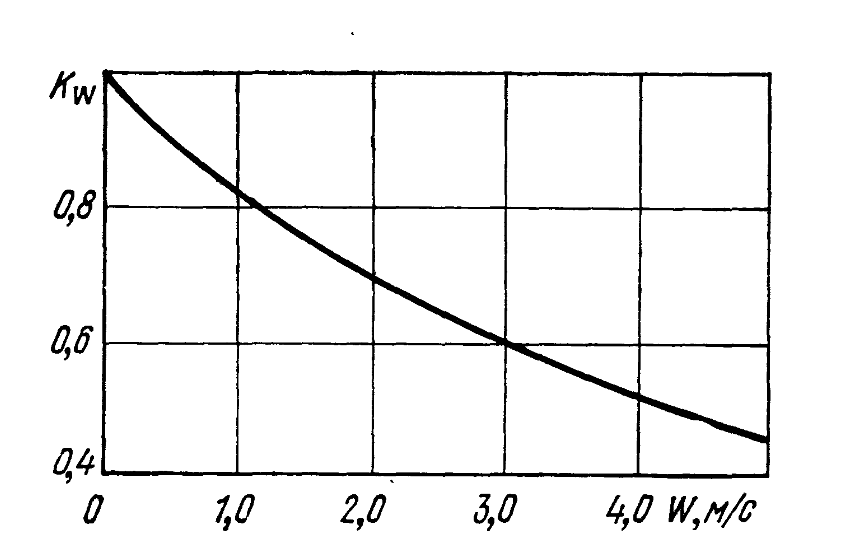
\includegraphics[scale=0.5]{Rotkop_pic_4.10.png}
  \caption{Зависимость $K_W$ от скорости
перемешивания~\cite{Rotkop1976}. }
\end{figure}

\item Определяется перегрев корпуса блока:
$$\vartheta\mathrm{_к} = 1,936 K$$
\item Определяется перегрев нагретой зоны \cite{Rotkop1976}:
  \begin{equation}
    \vartheta\mathrm{_з} = \vartheta_1 \cdot (K\mathrm{_{Н1}} - 1) + \vartheta_2 K_w
  \end{equation}
$$    \vartheta\mathrm{_з} = 4,927 K$$

\item Определяется средний перегрев воздуха в блоке ~\cite{Rotkop1976}:
  \begin{equation}
    \vartheta\mathrm{_в} = 0,75 \cdot \vartheta\mathrm{_з}
  \end{equation}

  $$\vartheta\mathrm{_в} = 3,695K$$
\item Находится удельная мощность элемента~\cite{Rotkop1976}:
  $$q\mathrm{_{эл}} =73,93\mathrm{ВТ/м^2} $$
\item Рассчитывается перегрев поверхности элемента ~\cite{Rotkop1976}:
  $$\vartheta\mathrm{_{эл}} =7,67$$

\item Рассчитывается перегрев окружающей элемент среды ~\cite{Rotkop1976}:
  $$\vartheta\mathrm{_{эс}} = 5,725K $$
  
\item Находится температура корпуса блока ~\cite{Rotkop1976}:
  $$T\mathrm{_{к}} = 314,936 K$$
\item Находится температура нагретой зоны, поверхности элемента,
    средняя температура в блоке и температура окружающей среды:
    $$T\mathrm{_з} = 317,927 K$$
    $$T\mathrm{_{эл}} = 320,670 K$$
    $$T\mathrm{_{в}} = 316,695 K$$
    $$T\mathrm{_{эс}} =318,752 K$$

    
\end{enumerate}